\section{Programming}

\subsection{Language and Libraries}
The video game was programmed using the object-oriented programming language C++. As the purpose of this project was to get familiar with modern C++, many features from the latest C++ standards (C++11/14/17/20) were used such as: classes, heritage, polymorphism...\\
The Standar Template Library is a C++ library used to enhance C++. Among other things, it contains very efficient and programmer-friendly containers and algorithms. These elements were massively used in order to create an efficient and readable program.\\
C++ does not natively provide functions to handle on screen display but the Simple DirectMedia Layer is a fairly easy to use library that provides all the objects and functions to easily handle 2D display.\\

\subsection{Programming Agreements}
In order to work efficiently as a team, some agreements regarding the repository and code organisation must be made.

The repository contains five main folders: \path{include}, \path{src}, \path{assets}, \path{build} and \path{doc}. The first one contains all the header files while the second one contains the corresponding source files (ie: \path{.cpp} files). The \path{assets} folders contains the sprites used in the game and the files representing levels. The two last folders are created and filled when building the project. After compiling, \path{build} contains the executable file and \path{doc} contains an \textit{html} documentation generated with Doxygen.\cite{doxygen}\\
The \path{include} and \path{src} contains the same file tree that corresponds to the objects'hierarchy. For instance, all files related to \textsf{Ghost} objects can be found in \path{game/object/moveable/ghosts}.

Throughout the entire project, the following naming scheme was used:
\begin{itemize}
    \item Pascal Case: classes, struct, enum and name spaces (except \textsf{LOG} to make it stands out in the code)
    \item Camel Case: functions and methods
    \item Serpent Case: variables and attributes (with an extra "_" at the end for classes attributes)
\end{itemize}

A dedicated header file is used to store all constants by declaring them using \textsf{constexpr} and encapsulated name spaces following the hierarchy. For instance the size of a \textsf{Ghost} can be accessed in every other file using: \textsf{gconst::game::game::object::moveable::ghost::size}.

All files were formated using the C/C++ VSCode extension from Microsoft and code documentation was generated by the Doxygen Documentation Generator VSCode extension.\cite{cpp_tools}\cite{gen_doc} In an effort to keep the code readable, explicit functions like constructors, destructors, \textit{getters} and \textit{setters} do not have documentation.
Additionnaly, all header files starts with a the preprocessing directives to include the file only once, followed by general imports then imports related to the project. In the same maner, source files start by including their associated header file.

\subsection{C++ Features}
The entire program relies on classes. From the \textsf{Application} to the small \textsf{Gommes} every element has been programmed as a class. For instance, the class \textsf{LOG} implements a logger. Using heritage, it is easy to add features to a class whitout starting from scratch. Following the afore mentionned file hierarchy, the class \textsf{Ghost} is a sub-class of \textsf{Moveable} which itself derives from \textsf{Object}. (Figure \ref{class_hierarchy})\\
Some classes are virtual meaning they contain virtual function(s) that must be implemented by the sub-class. For instance \textsf{Moveable} is a virtual class as it does not represent a real game object and contains among other \textsf{move} which is a virtual function. The definition of this method can be found either in \textsf{PacMan} or in \textsf{Ghost}, the two classes that inherits from \textsf{Moveable}.

\begin{figure}
    \center
    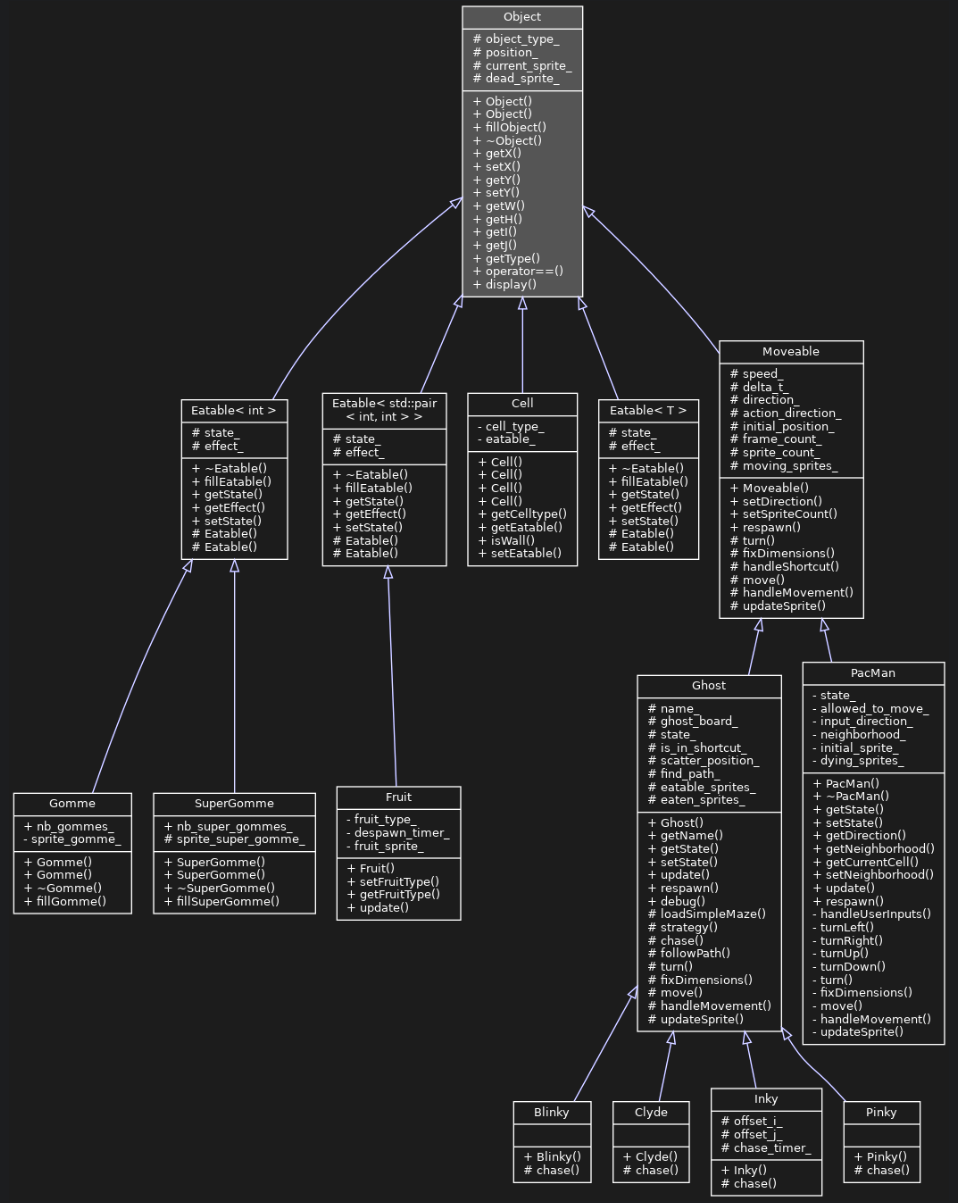
\includegraphics[scale=.25]{img/class_hierarchy.png}
    \caption{Game objects class hierarchy}
    \label{class_hierarchy}
\end{figure}

\textsf{Ghost} objects contains a \textsf{PathFinder} attribute to find the best path leading to the target position. This attribute is a \textit{functor}, that is to say an object used as a function by overloading the \textit{()} operator.

Game object that can be eaten by Pac-Man have an \textsf{effect\_} attribute that is used to apply an effect to the game (namely, update the score). This object is a \textit{lambda function}.

An particular attention has been paid to \textsf{public}, \textsf{protected} and \textsf{private} sections in order restrict access to object attributes and methods and improving code reliability. In the same maner, \textsf{const} marker is used to avoid programming errors.

\subsection{Standard Template Library Features}
During the entire game, a single object of the class \textsf{Fruit} is created and updated, that is to say: its \textsf{fruit\_type\_} attributes is set to the correct fruit. In order to keep the lambda function, the \textsf{Eatable} class was templated: \textsf{Gommes} are \textsf{Eatable\<int\>} (the lambda function takes a single integer argument that corresponds to the current score and returns the new score) and \textsf{Fruit} are \textsf{Eatable\<std::pair\<int,int\>\>} (the lambda function takes a pair of interger as argument where the first value is the score of the game and the second value is a array index used to add the value corresponding to a fruit to the score).

All containers are \textsf{std::array} or \textsf{std::vector}. For instance in the class \textsf{Game} the \textsf{board\_} attributes used to represent the game board is a two dimentional array made by creating an array of arrays (see name space \textsf{Board}).

\textsf{std::pair} are used to represent positions on the board for all methods and attributes related to the movement of the \textsf{Ghost} objects and in the \textsf{effect\_} lambda function of \textsf{Fruit} as seen before.

All text objects are of type \textsf{std::string}.

Using this containers allows to use operators (\textsf{==}, \textsf{std::min}...) and pre-emplemented algorithms such as \textsf{find}, \textsf{fill} and \textsf{tolower}.

The \textsf{PathFinder} functor required priority queues to implement the Astar algorithm.\cite[astar] However, \textsf{std::priority\_queue} does not implement the \textsf{find} method. Using templates, another priority queue implementing the \textsf{find} method has been created \textsf{std::priority\_queue}. (See  \textsf{PriorityQueue})

\subsection{SDL Features}
The SDL was used in order to create a window to display the game inside. Special functions used to initialise and quit the SDL, load and unload image assets are declared in \path{SDL\_utils.h} and \path{SDL\_utils.cpp} files.

The \textsf{SDL\_BlitScaled} function is used to display sprites. Additionnaly, the \textsf{SDL\_FillRect} function was used to draw object bouding boxes during developement.

A simple timer relying on the \textsf{SDL\_GetTicks64} has been implemented as a class (\textsf{Timer}).

\subsection{Game Reproduction}
The goal of this project is to recreate the original Pac-Man game from 1980. Eventhough the game looks really simple, this is not an easy task as every object has multiple states, actions or effect.

Starting with the main character, the main difficulty was to properly handle the movement as it can move continuously on a discrete environnement. In other words, there is always one dimension that is fixed: if \textsf{PacMan} is moving to the left, its y coordinate is fixed to a precise value. Moreover, \textsf{PacMan} can cut corners to enhance playability. To do that we created an object called \textsf{Cell} representing a cell in the maze thus discretizing the board. \textsf{Cell} objects are used to keep track of the cells around \textsf{PacMan} so it is easy to look for walls.

\textsf{Ghost} movement is also difficult to implement as it is not relying on user input but rather on an artifical intelligence. According to its state a \textsf{Ghost} move to a specified target position by following the shortest path. In order to do that, the Astar algorithm has been implemented in the \textsf{PathFinder} class. However, there are constrains that can forbid the \textsf{Ghost} to follow the best path (ie: a \textsf{Ghost} cannot make a 180 degree turn). So if it cannot go in the best computed direction, the \textsf{Ghost} simply follow the walls.\\
In the original game, every single ghost has its own strategy to chase Pac-Man. Each of the \textsf{Ghost} sub-class redefines the \textsf{chase} method: \textsf{Blinky} (red) directly chase \textsf{PacMan}, \textsf{Inky} (blue) has a target randomly choosen around \textsf{PacMan} and \textsf{Clyde} (orange) and \textsf{Pinky} (pink) try to go four cells in front/behind \textsf{PacMan}.

Every type of eatable object from the original game are implemented. \textsf{Gommes} and \textsf{SuperGommes} classes correspond to the dots pac-man can eat all over the maze and \textsf{Fruit} represent the fruit that appears at given score values.

The overlay uses \textsf{PacString} to display information. This simple class convert a string into an \textsf{Object} that can be easily displayed on the game window.

Level changements as weel as the end of the game are properly recreated and bug-free.

\begin{figure}
    \center
    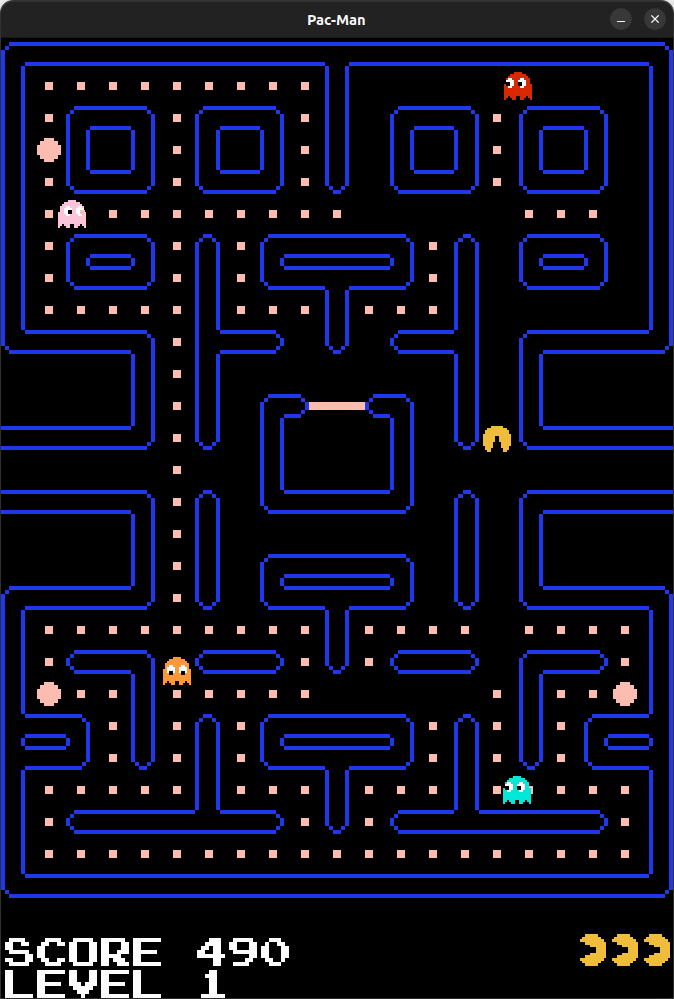
\includegraphics[scale=.25]{img/game.png}
    \caption{Game screenshot}
    \label{game}
\end{figure}